\documentclass[UTF8]{article}
%\usepackage{natbib}
\usepackage{geometry}                % See geometry.pdf to learn the layout options. There are lots.
\geometry{a4paper}                   % ... or a4paper or a5paper or ... 

%\geometry{landscape}                % Activate for for rotated page geometry
\usepackage{breakurl}     
\usepackage{graphicx}
\usepackage{graphbox}
\usepackage{hyperref}
\usepackage{amssymb}
\usepackage{epstopdf}
\usepackage{algorithm}
\usepackage{amsmath}
\usepackage[noend]{algpseudocode}
\usepackage{enumitem}
\usepackage[acronym]{glossaries}
\usepackage[hang,footnotesize,bf]{caption}
\DeclareGraphicsRule{.tif}{png}{.png}{`convert #1 `dirname #1`/`basename #1 .tif`.png}

% Copied from StackOverflow for code snippets 
% ------------------------------------------------------------
\usepackage{listings}
\usepackage{color}

\definecolor{dkgreen}{rgb}{0,0.6,0}
\definecolor{gray}{rgb}{0.5,0.5,0.5}
\definecolor{mauve}{rgb}{0.58,0,0.82}

\lstset{frame=tb,
  language=Python,
  aboveskip=3mm,
  belowskip=3mm,
  showstringspaces=false,
  columns=flexible,
  basicstyle={\small\ttfamily},
  numbers=none,
  numberstyle=\tiny\color{gray},
  keywordstyle=\color{blue},
  commentstyle=\color{dkgreen},
  stringstyle=\color{mauve},
  breaklines=true,
  breakatwhitespace=true,
  tabsize=3
}


% Copied from Stack Exchange for ToDo items
% -----------------------------------------------------------
\usepackage{xargs} 
\usepackage[pdftex,dvipsnames]{xcolor}  % Coloured text etc.
% 
\usepackage[colorinlistoftodos,prependcaption,textsize=tiny]{todonotes}
\newcommandx{\unsure}[2][1=]{\todo[linecolor=red,backgroundcolor=red!25,bordercolor=red,#1]{#2}}
\newcommandx{\change}[2][1=]{\todo[linecolor=blue,backgroundcolor=blue!25,bordercolor=blue,#1]{#2}}
\newcommandx{\info}[2][1=]{\todo[linecolor=OliveGreen,backgroundcolor=OliveGreen!25,bordercolor=OliveGreen,#1]{#2}}
\newcommandx{\improvement}[2][1=]{\todo[linecolor=Plum,backgroundcolor=Plum!25,bordercolor=Plum,#1]{#2}}
\newcommandx{\feedback}[2][1=]{\todo[linecolor=Goldenrod,backgroundcolor=Goldenrod!25,bordercolor=Coldenrod,#1]{#2}}
\newcommandx{\thiswillnotshow}[2][1=]{\todo[disable,#1]{#2}}


\title{Validator Economics: Variable min validator deposit size\\
\vspace{4pt}
\large EF Academic Grant ID: FY23-1030\\
\vspace{16pt}
DRAFT MODEL, CHALLENGES \& POTENTIAL MITIGATIONS\\
(MAXEB - EIP-7521) }
\vspace{16pt}
\author{Sandra Johnson\\
Consensys Software R\&D}
\date{\today}                                           % Activate to display a given date or no date

\begin{document}
\maketitle


% Acronym definitions
\newacronym{apr}{APR}{annual percentage rate}
\newacronym{bls}{BLS}{Boneh–Lynn–Shacham}
\newacronym{bn}{BN}{Bayesian network}
\newacronym{cbeth}{cbETH}{Coinbase wrapped staked ETH}
\newacronym{cdf}{CDF}{cumulative distribution function}
\newacronym{cl}{CL}{consensus layer}
\newacronym{cpt}{CPT}{conditional probability table}
\newacronym{dos}{DoS}{denial of service}
\newacronym{dvt}{DVT}{distributed validator technology}
\newacronym{eb}{EB}{effective balance}
\newacronym{ef}{EF}{Ethereum Foundation}
\newacronym{eip}{EIP}{Ethereum Improvement Proposal}
\newacronym{el}{EL}{execution layer}
\newacronym{epbs}{ePBS}{enshrined PBS}
\newacronym{ffg}{FFG}{Friendly finality gadget}
\newacronym{fxs}{FXS}{Frax share}
\newacronym{ghost}{GHOST}{Greedy Heaviest-Observed Sub-Tree}
\newacronym{ldo}{LDO}{Lido DAO}
\newacronym{lmd}{LMD}{Latest message driven}
\newacronym{mev}{MEV}{maximal extractable value}
\newacronym{mm}{MM}{MetaMask}
\newacronym{npt}{NPT}{node probability table}
\newacronym{p2p}{p2p}{peer-to-peer}
\newacronym{pbs}{PBS}{proposer builder separation}
\newacronym{pc}{PC}{personal computer}
\newacronym{pdf}{PDF}{probability density function}
\newacronym{pos}{PoS}{proof of stake}
\newacronym{pr}{PR}{pull request}
\newacronym{rig}{RIG}{Robust Incentives Group}
\newacronym{rpl}{RPL}{Rocket Pool}
\newacronym{ssf}{SSF}{single-slot finality}
\newacronym{steth}{stETH}{Lido staked Ether}
\newacronym{ups}{UPS}{uninterruptable power supply}
\newacronym{vrf}{VRF}{verifiable random function}

% ------------------------------------------------------------------------------
\section{Overview}
% ------------------------------------------------------------------------------
This document builds on the previous document, \textit{Milestone 1(EB): Review \& analyse EIP-7521}, addressing each of the identified challenges and applying example scenarios to the expected behaviour cited in blog posts and analysis done to date.

In summary, as mentioned in the previous document, the two key criteria we need to assess for this proposal, and indeed for any proposed strategy to reduce, or cap, the validator set size, are the risks and benefits introduced by that proposal. \\

\noindent
With respect to EIP-7521:
\begin{itemize}
\item \textbf{Risks}: Are risks are being introduced by this proposal? Are there adverse affects on some categories of stakers, or the Ethereum ecosystem?
\item  \textbf{Benefits}: Do all staker categories benefit equally from EIP-7521? Apart from the expected reduction in network load, are there other benefits to the health of the ecosystem?
\end{itemize}

We need to bear in mind that regardless of the risks and benefits, EIP-7521 relies on stakers' willingness to consolidate at least some of their validators. Therefore the messaging around the benefits of consolidation and the perception that the benefits to stakers and the ecosystem definitely outweigh any perceived risks needs to be compelling.

The impact on staking pools, their operational business models, and software changes required to take advantage of the increased maximum will need to be discussed with stakeholders \gls{eb}.

Mike Neuder summarised several concerns and potential problems if the MaxEB proposal is not implemented in the next hard fork:\\
\noindent
Without MaxEB:
\begin{itemize}
\item risk of massive influx of staking demand making the total validator count pushing the safety limits of the network
\item risk of extending the earliest timeline for \gls{ssf} because consolidation may be a slow process that we need to start
\item slightly more pooling pressure from solo stakers because there are no variable balances
\item risk of longer time until we could drop the min effective balance because validator count is too high
\end{itemize}

\clearpage
% -------------------------------------------------------------------------------------
\section{Challenges \& Additional analysis requirements}
% -------------------------------------------------------------------------------------
\label{sec:challenges}
In addition to the advantages and disadvantages highlighted in the \textit{ethresear.ch} post, \href{https://ethresear.ch/t/increase-the-max-effective-balance-a-modest-proposal/15801/3}{\textit{Increase the MAX\_EFFECTIVE\_BALANCE – a modest proposal}}, by  Neuder et al  \cite{Neuder2023a}, we propose three topics that may benefit from further in-depth analysis and working examples:

\begin{itemize}
\item Validator duty selection
\thiswillnotshow [inline] {Previously this was "Committee participation"}
\item Rewards \& penalties
\item Ethereum ecosystem \& protocol
\end{itemize}

Each of the three topics will be discussed in more detail. 

% ----------------------------------------------
\subsection{Validator duty selection}
% ----------------------------------------------
In this section we review each of the selection processes to confirm or challenge the anticipated behaviour.

\begin{enumerate}

\item \textit{Proposer selection}: demonstrate that proposer selection still works as designed with partial and full consolidation of validators.

\item \textit{Sync committee selection}: demonstrate that sync committee selection will work as designed even when there is a large increase in Max\gls{eb}.

\item \textit{Slot committees}: Demonstrate that not taking validator weight into account does not have any adverse downstream effects. D'Amato and Neuder state that even if one ``attestation is majority adversarial'', then the worst that can happen is that the attacker will execute a local reorg \cite{damato2023}. Explore in more detail, e.g. use an example or two, to ascertain the effect of variations in slot committee balances with the inclusion, or omission, of fully consolidated stakers. 

\item \textit{Aggregator selection}: Does the selection of more than one virtual validator of a consolidated validator change the probability distribution of sub-committees? Could the probability of fewer than 16 distinct aggregators increase? \\
\textit{Virtual validators}: D'Amato and Neuder's conjecture is that treating consolidated validators as several `virtual' validators yields two main benefits \cite{damato2023}. Demonstrate the correctness of these statements.:
	\begin{itemize}
	\item The total number of aggregators is unchanged, because one consolidated validator would account for only one aggregator.
	\item The probability of at least one honest validator is equivalent to the current probability, because the introduction of virtual validators means that the probability of selecting an honest aggregator is the same as it is currently. The total number of honest validators prior to EIP-7251 is the same as the number of virtual and unconsolidated honest validators.
	\end{itemize}
	
\end{enumerate}


% ----------------------------------------------
\subsection{Rewards \& penalties}
% ----------------------------------------------
\begin{enumerate}

\item \textit{Proposer selection probability}: Demonstrate that this  probability remains unchanged and will not unduly disadvantage small-scale solo stakers \cite{Neuder2023a}. 

\item \textit{Whistleblower reward}: Currently the proposer receives both the whistleblower reward and the proposer reward. Moreover, the whistleblower reward is proportional to the slashed validator's effective balance. How is this reward influenced by the increased maximum effective balance?	

\item \textit{Slashing penalties}: Verify the suitability of the suggested changes to slashing penalties (initial and correlation penalties), as well as those penalties remaining unchanged (attestation and inactivity leak penalties), proposed by Neuder and Monnot \cite{Neuder2023d} using working examples, or other approaches.\\
Moreover, based on the severity of the changed slashing penalties, what situation constitutes an attack on the chain? How do we assess whether the penalties are sufficient to deter adverse behaviour? Are the proposed changes too lenient for large stakers?


\end{enumerate}

% ----------------------------------------------
\subsection{Ethereum ecosystem \& protocol}
% ----------------------------------------------
It is important that there no adverse impacts on the health of the Ethereum ecosystem, and a lot of analysis has already been undertaken to ensure that it remains secure and healthy. As a consequence of EIP-7521, as with all EIPs, changes to the protocol would be required, which the initiators of the proposal have endeavoured to minimise.

\begin{enumerate}

\item \textit{Worst case: Full consolidation}: D'Amato and Neuder identify full consolidation as the worst case scenario when we consider two groups of validators: honest and adversarial validators. Several reasons are given for this conclusion \cite{damato2023}. Using examples or other approaches we need to check the veracity of these statements, viz. that full consolidation:
	\begin{itemize}
	\item increases the probability that one or more committees will be majority dishonest
	\item increases the variance of adversarial balances
	\item increases the variance of the distribution of adversarial weight over committees
	\item due to the above, it follows that it is more likely that there will be ``a positive deviation from the expected adversarial weight in a committee''. Apparently although there may also be ``negative deviations'' the adversarial party is not concerned because it merely aims to control at least one committee.
	\item On the other hand, full consolidation of honest validators maximises the risk of negative deviations from the expected committee weight.
	\item Honest validators benefit from spreading weight evenly across the committees because it minimises the risk of negative deviations.
	\end{itemize}


\item \textit{Discouragement attacks}: Investigate potential griefing, or discouragement, attacks.

\item \textit{Consolidating validators}: There are many challenges around exiting and activation of validators for consolidation. Therefore, as Asgaonkar points out, in-protocol consolidation needs to be in place \cite{Asgaonkar2023}.

\item \textit{Withdrawals}: The automated withdrawal sweep will now skip over consolidated validators with an effective balance below 2, 048 ETH. Therefore, there may be reductions in time to do a full sweep as well as a reduced network load because fewer withdrawals will be initiated. \\
The capability of being able to initiate partial withdrawals for a specified amount appears to be a requirement of large staking pools such as Lido.

\item \textit{Centralisation forces}: 
Centralisation needs to be assessed within the context of this grant and the proposed increase in maximum effective balance, especially with respect to large stakers and staking pools.

\item \textit{Bayesian network model}: Build a \gls{bn} to capture current factors and interactions, including distributions around factors such as uptake of consolidation, current distribution of different categories of stakers, etc. \\
Use the \gls{bn} model to gain insight into questions such as:
	\begin{itemize}
	\item What does the landscape look like if there is no consolidation, but some or all validators decide to compound their rewards? Is this a good or desirable outcome? 
	\item Create some example scenarios that include solo, partial and fully consolidated stakers and how different compositions translate to the selection of validators for specific duties and ideally the probability of dishonest committees.
	\end{itemize}
 
\end{enumerate}

In summary it is important to ensure that small scale solo-stakers are not unduly disadvantaged with the introduction of a 2,048 ETH MaxEB, in terms of proposer selection etc. which may disincentivise the commitment to running a validator. What is being compromised to enable consolidation? Are there other aspects we have not considered? What are the negatives for solo stakers who are considered to be the backbone of Ethereum? Does MaxEB swing it too much in favour of large stakers? One important advantage for solo stakers is that any rewards earned can be autocompounded and if they have insufficient ETH to activate another validator, they can instead top up their validator(s) with amounts less than 32 ETH, e.g. 5 ETH.


% ------------------------------------------------
% ===============
\section{Analysis - TO DO}
% ===============
\label{sec:analysis}
% -------------------------------------------------------------
\subsection{Validator duty selection}
% ------------------------------------------------------------
The selection of validators to be part of committees or to be selected as a proposer needs to be done in an unpredictable, or random, way to ensure that the selection cannot be manipulated by bad actors.

However, in a blockchain system, all nodes need to come to consensus, and the key ``randomness lever'' is the seed used in the  calculation that would have the same outcome for all nodes. Therefore the seed needs to be unpredictable \cite{buterin2020}.



In the Consensus Layer there are a few different approaches to achieve randomness used in selection of validators for duties:
\begin{itemize}
\item Aggregators are selected via a \gls{vrf} lottery \cite{Edgington2023}.
\end{itemize}


% ------------------------------------------------
\subsubsection*{Proposer}
% ------------------------------------------------
Endianness, the order of bytes in the binary representation of a number, is not commonly of interest, but in the case of index shuffling and proposer selection, the RANDAO, and serialising with SSZ, the endianness does matter. Initially big-endian was used, i.e. the first byte is the most-significant byte, but this has now changed mainly to little-endian, i.e. the first byte is the least-significant byte \cite{Edgington2023}.

% From. Ben's book: https://eth2book.info/capella/part3/helper/misc/#compute_proposer_index

% Mike Neuder links to the compute_proposer_index method: https://github.com/ethereum/consensus-specs/blob/9c35b7384e78da643f51f9936c578da7d04db698/specs/phase0/beacon-chain.md#compute_proposer_index 
% in his "Increase the MAX_EFFECTIVE_BALANCE – a modest proposal" blog: https://ethresear.ch/t/increase-the-max-effective-balance-a-modest-proposal/15801


The \textit{swap-or-not-shuffle} technique \cite{hoang2014}  is used to shuffle the validator indices in preparation for the selection of a block proposer. This is done in \href{https://github.com/ethereum/consensus-specs/blob/9c35b7384e78da643f51f9936c578da7d04db698/specs/phase0/beacon-chain.md#compute_shuffled_index}{\textit{compute\_shuffled\_index}}.

The computation to determine the proposer for the next block is done in \href{https://github.com/ethereum/consensus-specs/blob/9c35b7384e78da643f51f9936c578da7d04db698/specs/phase0/beacon-chain.md#compute_proposer_index}{\textit{compute\_proposer\_index}}: 

\lstset{language=Python}

\begin{lstlisting}
def compute_proposer_index(state: BeaconState, indices: Sequence[ValidatorIndex], seed: Bytes32) -> ValidatorIndex:
    """
    Return from ``indices'' a random index sampled by effective balance.
    """
    assert len(indices) > 0
    MAX_RANDOM_BYTE = 2**8 - 1
    i = uint64(0)
    total = uint64(len(indices))
    while True:
        candidate_index = indices[compute_shuffled_index(i % total, total, seed)]
        random_byte = hash(seed + uint_to_bytes(uint64(i // 32)))[i % 32]
        effective_balance = state.validators[candidate_index].effective_balance
        if effective_balance * MAX_RANDOM_BYTE >= MAX_EFFECTIVE_BALANCE * random_byte:
            return candidate_index
        i += 1
\end{lstlisting}


Therefore, we iterate through the shuffled indices, starting with the first entry and then check whether it passes the selection criteria. If it doesn't, then the next candidate index goes through the same checks.

The validator's effective balance is multiplied by 255 and then compared to the product of the generated \textit{random\_byte}, which we assume is uniformly randomly distributed across 0 to 255,  and the \textit{MAX\_EFFECTIVE\_BALANCE} which is now 2,048 ETH. 

Therefore the probability of a validator being the proposer if their index was selected from the list can be calculated as follows:
% , as indicated by Neuder in his \href{https://ethresear.ch/t/increase-the-max-effective-balance-a-modest-proposal/15801}{blog post} 

%We already weight the probability of becoming a proposer by the effective balance of that validator. See compute\_proposer\_index 17. Currently, if a validator’s effective balance (EB) is below the MaxEB, they are selected as the proposer given their validator index was randomly chosen only if,
\begin{equation}
\label{eqn:1}
\begin{split}
& P(proposer) = P(EB * 255 \geqslant MaxEB*r) \texttt{ } where \texttt{ } r \sim U(0,255), \textit{ } r = random\_byte, EB = \textit{validator effective balance} \\
& \therefore P(proposer) = P\left(r \leqslant \frac{255*EB}{MaxEB} \right) \\
& \therefore \textit{if } EB = MaxEB \implies P(proposer) = 1\\
\end{split}
\end{equation}
%
Therefore, if the effective balance of the candidate validator equalled the maximum effective balance, then the validator becomes the proposer with probability 1. 

This creates some interesting scenarios when the maximum effective balance is increased to 2,048 ETH. As before, a fully consolidated validator will become a proposer with a probability of 1 if the 
validator's index was randomly selected as the next candidate. 

\begin{equation*}
\begin{split}
& \textit{Given the candidate index belongs to a solo staker with an effective balance of 32 ETH, then } \\
& P(proposer) = P\left(r \leqslant \frac{255*32}{2048} \right) \\
& \therefore P(proposer) = P(r \leqslant 3.98) = \left(\frac{3.98-0}{255}\right) = 0.016\\
& \\
& \textit{Given the candidate index belongs to a staker with a partially consolidated validator (2 * 32 ETH) effective balance , then } \\
& P(proposer) = P\left(r \leqslant \frac{255*64}{2048} \right) \\
& \therefore P(proposer) = P(r \leqslant 7.97) = \left(\frac{7.97-0}{255}\right) = 0.031\\
& \\
& \textit{Given the candidate index belongs to a staker with a partially consolidated validator (5 * 32 ETH) effective balance , then } \\
& P(proposer) = P\left(r \leqslant \frac{255*160}{2048} \right) \\
& \therefore P(proposer) = P(r \leqslant 19.92) = \left(\frac{19.92-0}{255}\right) = 0.078\\
\end{split}
\end{equation*}


In other words, the probability of passing the check for selection to propose the next block is 1.6\% for an unconsolidated staker, 3.1\% for a validator with double the previous MaxEB, 7.8\% for a validator that has 5-fold the previous MaxEB (160 ETH), and the probability remains as 100\%, i.e. complete certainty that if a fully consolidated validator's index is selected as the next candidate, it will pass the proposer eligibility check.

Assuming a validator set size of 716,800, then
the probability of any validator being chosen as the candidate index for the next block proposer is: \\
$P(candidate) = \frac{1}{(Active \texttt{ } validator \texttt{ } set \texttt{ } size)} = \frac{1}{ 716,800} = 0.000001395$, or 0.0001395 \%. 

Previously, providing a validator maintained its effect balance at 32 ETH, once its index was selected as the next candidate, it would have passed the proposer selection test with certainty (probability of 1, i.e. 100\%).

Putting it another way:
\begin{equation*}
\begin{split}
& \textit{Given EB=32 ETH, then currently } \\
& P(candidate \& proposer) = P(candidate) * P(proposer) = 0.000001395 * 1 = 0.000001395 \\
& \textit{After MaxEB = 2048 ETH, this changes to:} \\
& P(candidate \& proposer) = 0.000001395 * 0.016 = 0.00000002232 \\
\end{split}
\end{equation*}

Let us look at some example scenarios, assuming an active validator set of 716,800 validators, i.e. a total deposit size of $716,800 * 32 ETH \approx 22.94$ \textit{M ETH}:
\begin{enumerate}
\item Validator set comprises only validators with an effective balance of 32 ETH.
\item Validator set comprises only validators that are fully consolidated, i.e. each validator has an effective balance of 2,048 ETH.
\item Validator set comprises a combination of validators: solo stakers, partially consolidated stakers and fully consolidated stakers.
\end{enumerate}

Interesting questions:
\begin{itemize}
\item What is the probability that no proposer is selected for a slot when no consolidation has yet happened? This situation could occur during implementation time, before stakers merge some or all of their validators.
\end{itemize}


\noindent
\textbf{\textit{Scenario 1}} \\
% -------------------
\noindent
In figure \ref{fig:random} on page \pageref{fig:random} we generated 716,800 random values from \textit{U(0,255)} \\

\begin{figure}[htbp]
\begin{center}
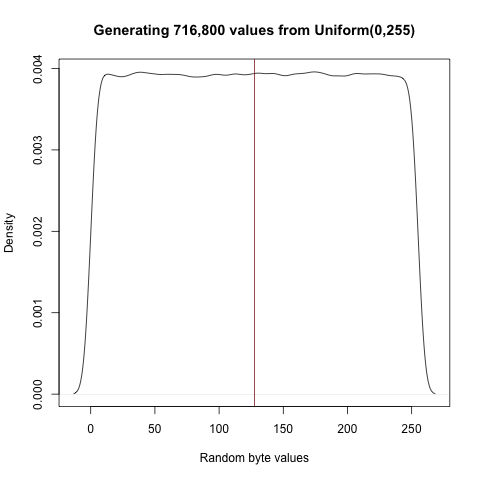
\includegraphics[width=0.5\linewidth]{images/validator-indices-density}
\caption{Distribution of 716,800 random bytes generated from U(0,255)}
\label{fig:random}
\end{center}
\end{figure}


\begin{figure}[htbp]
\begin{center}
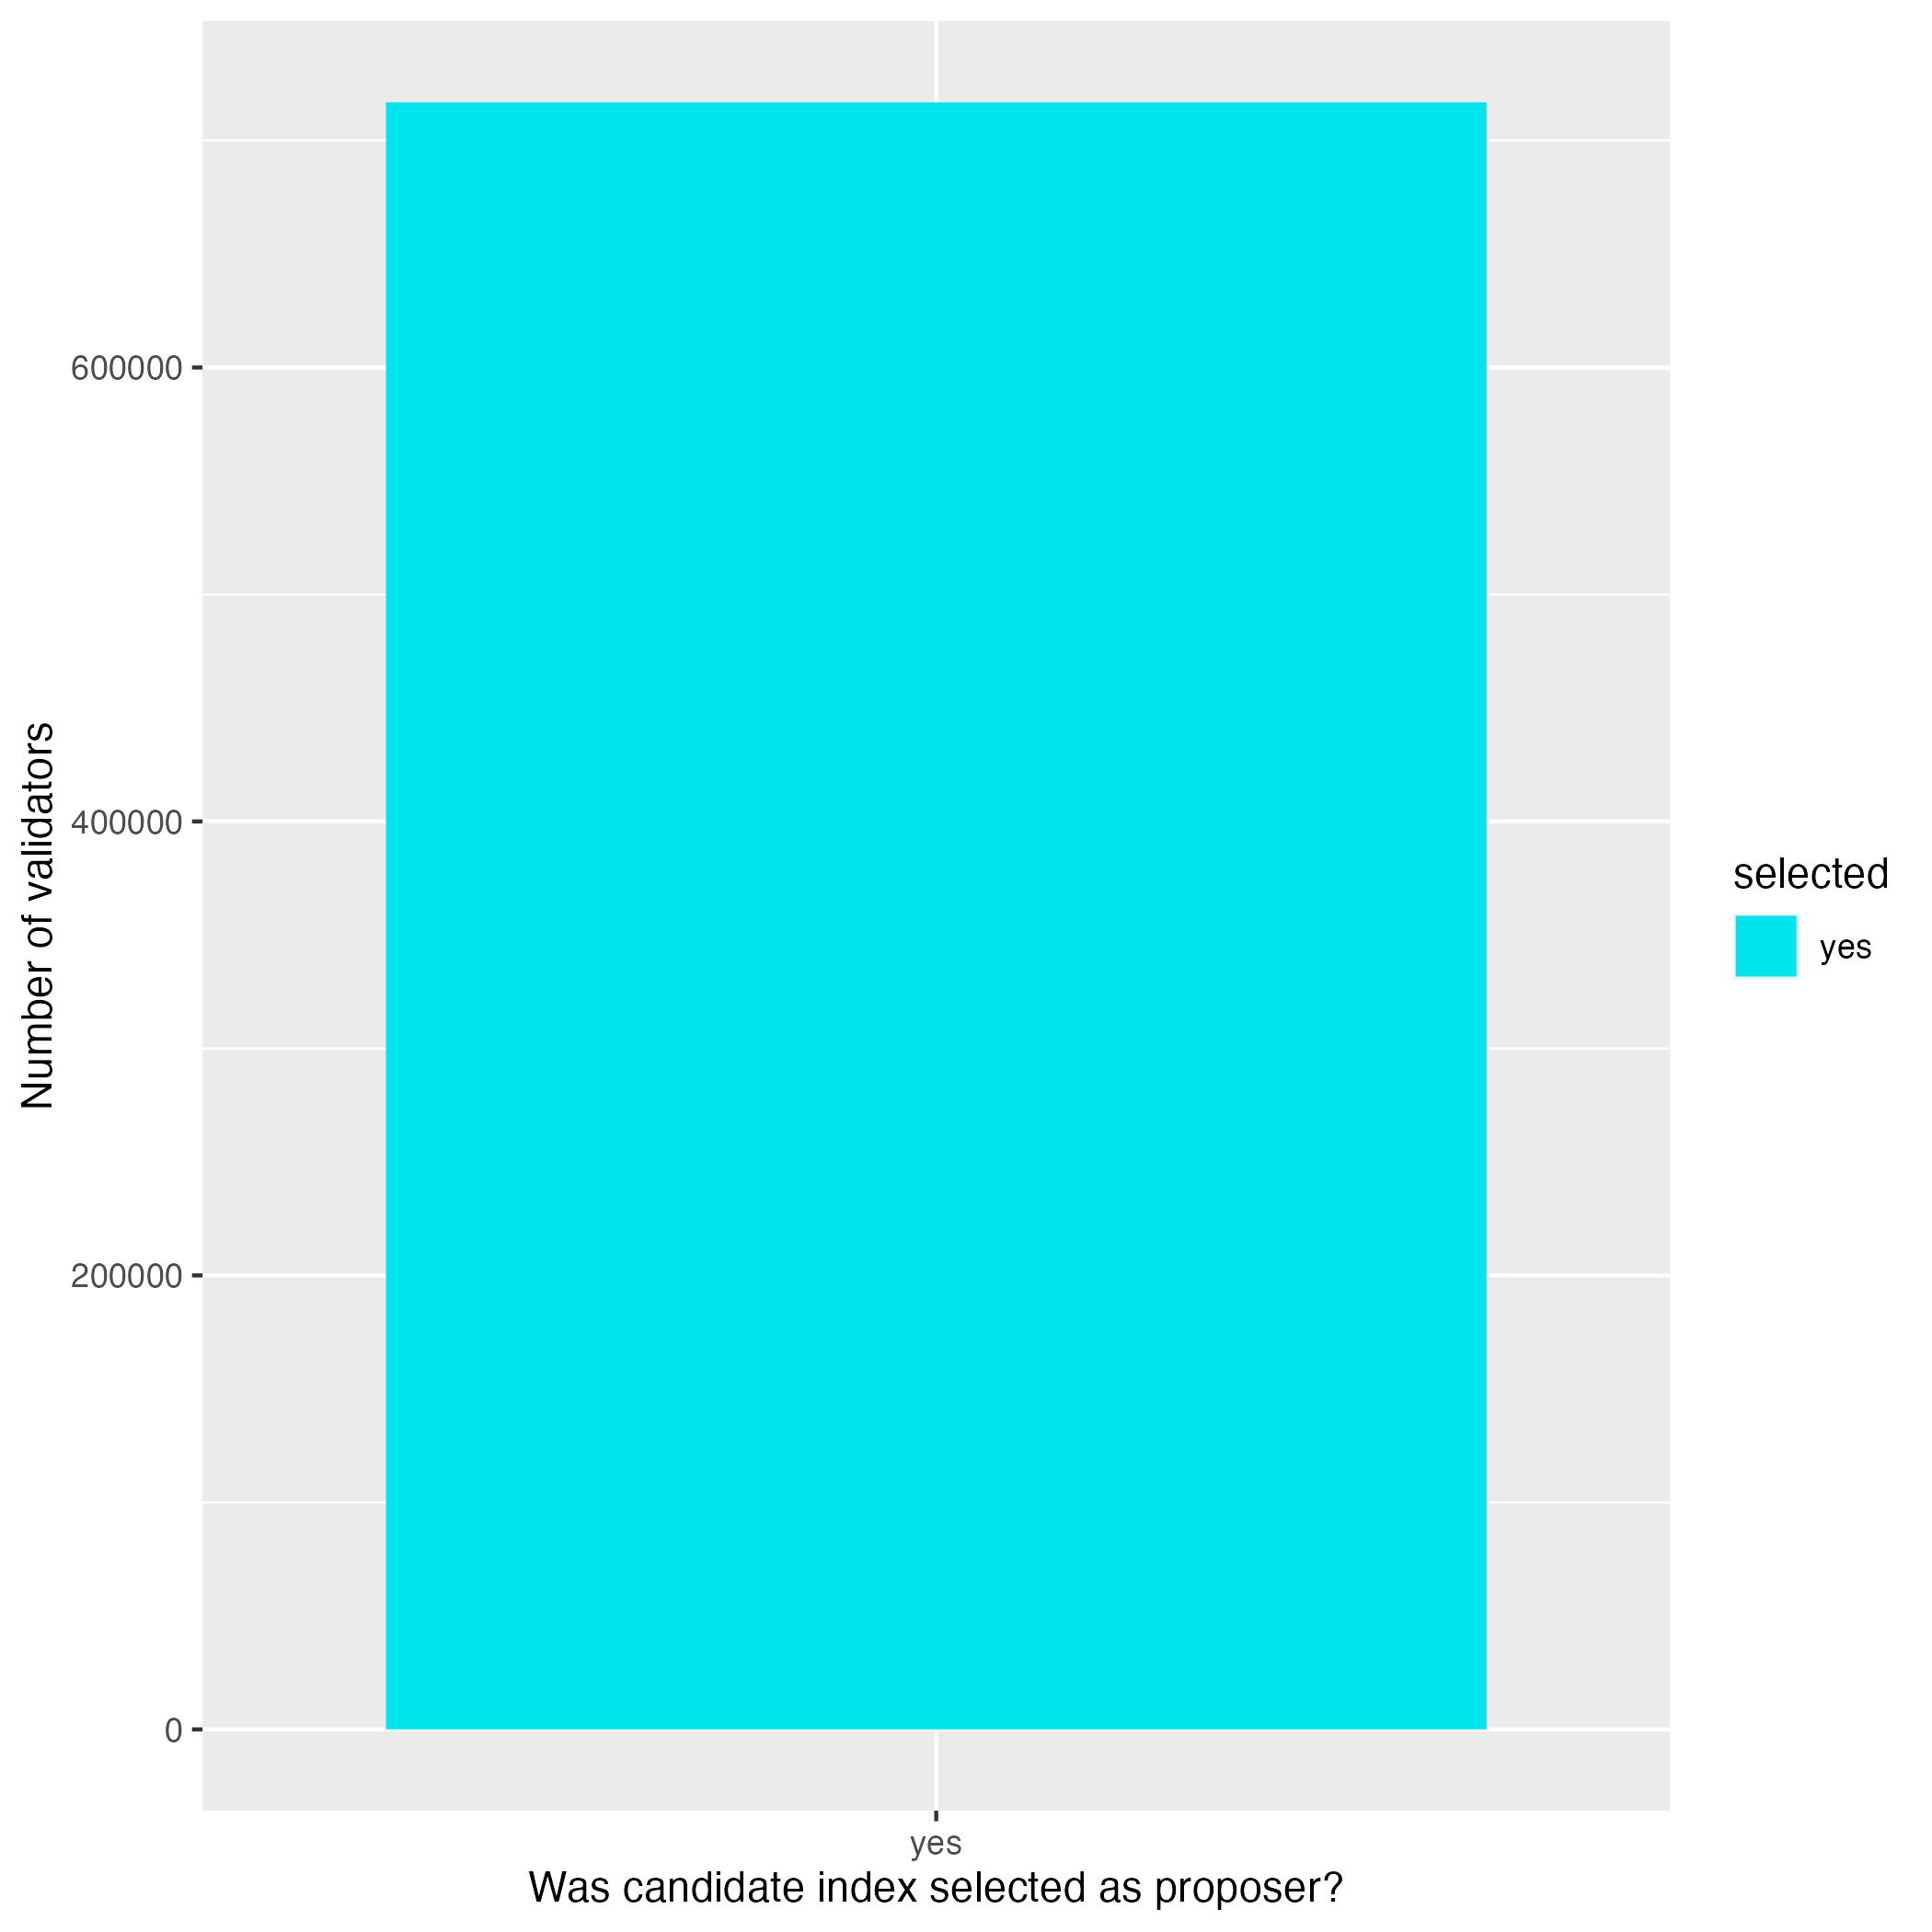
\includegraphics[width=0.45\linewidth]{images/current-solo-barchart}
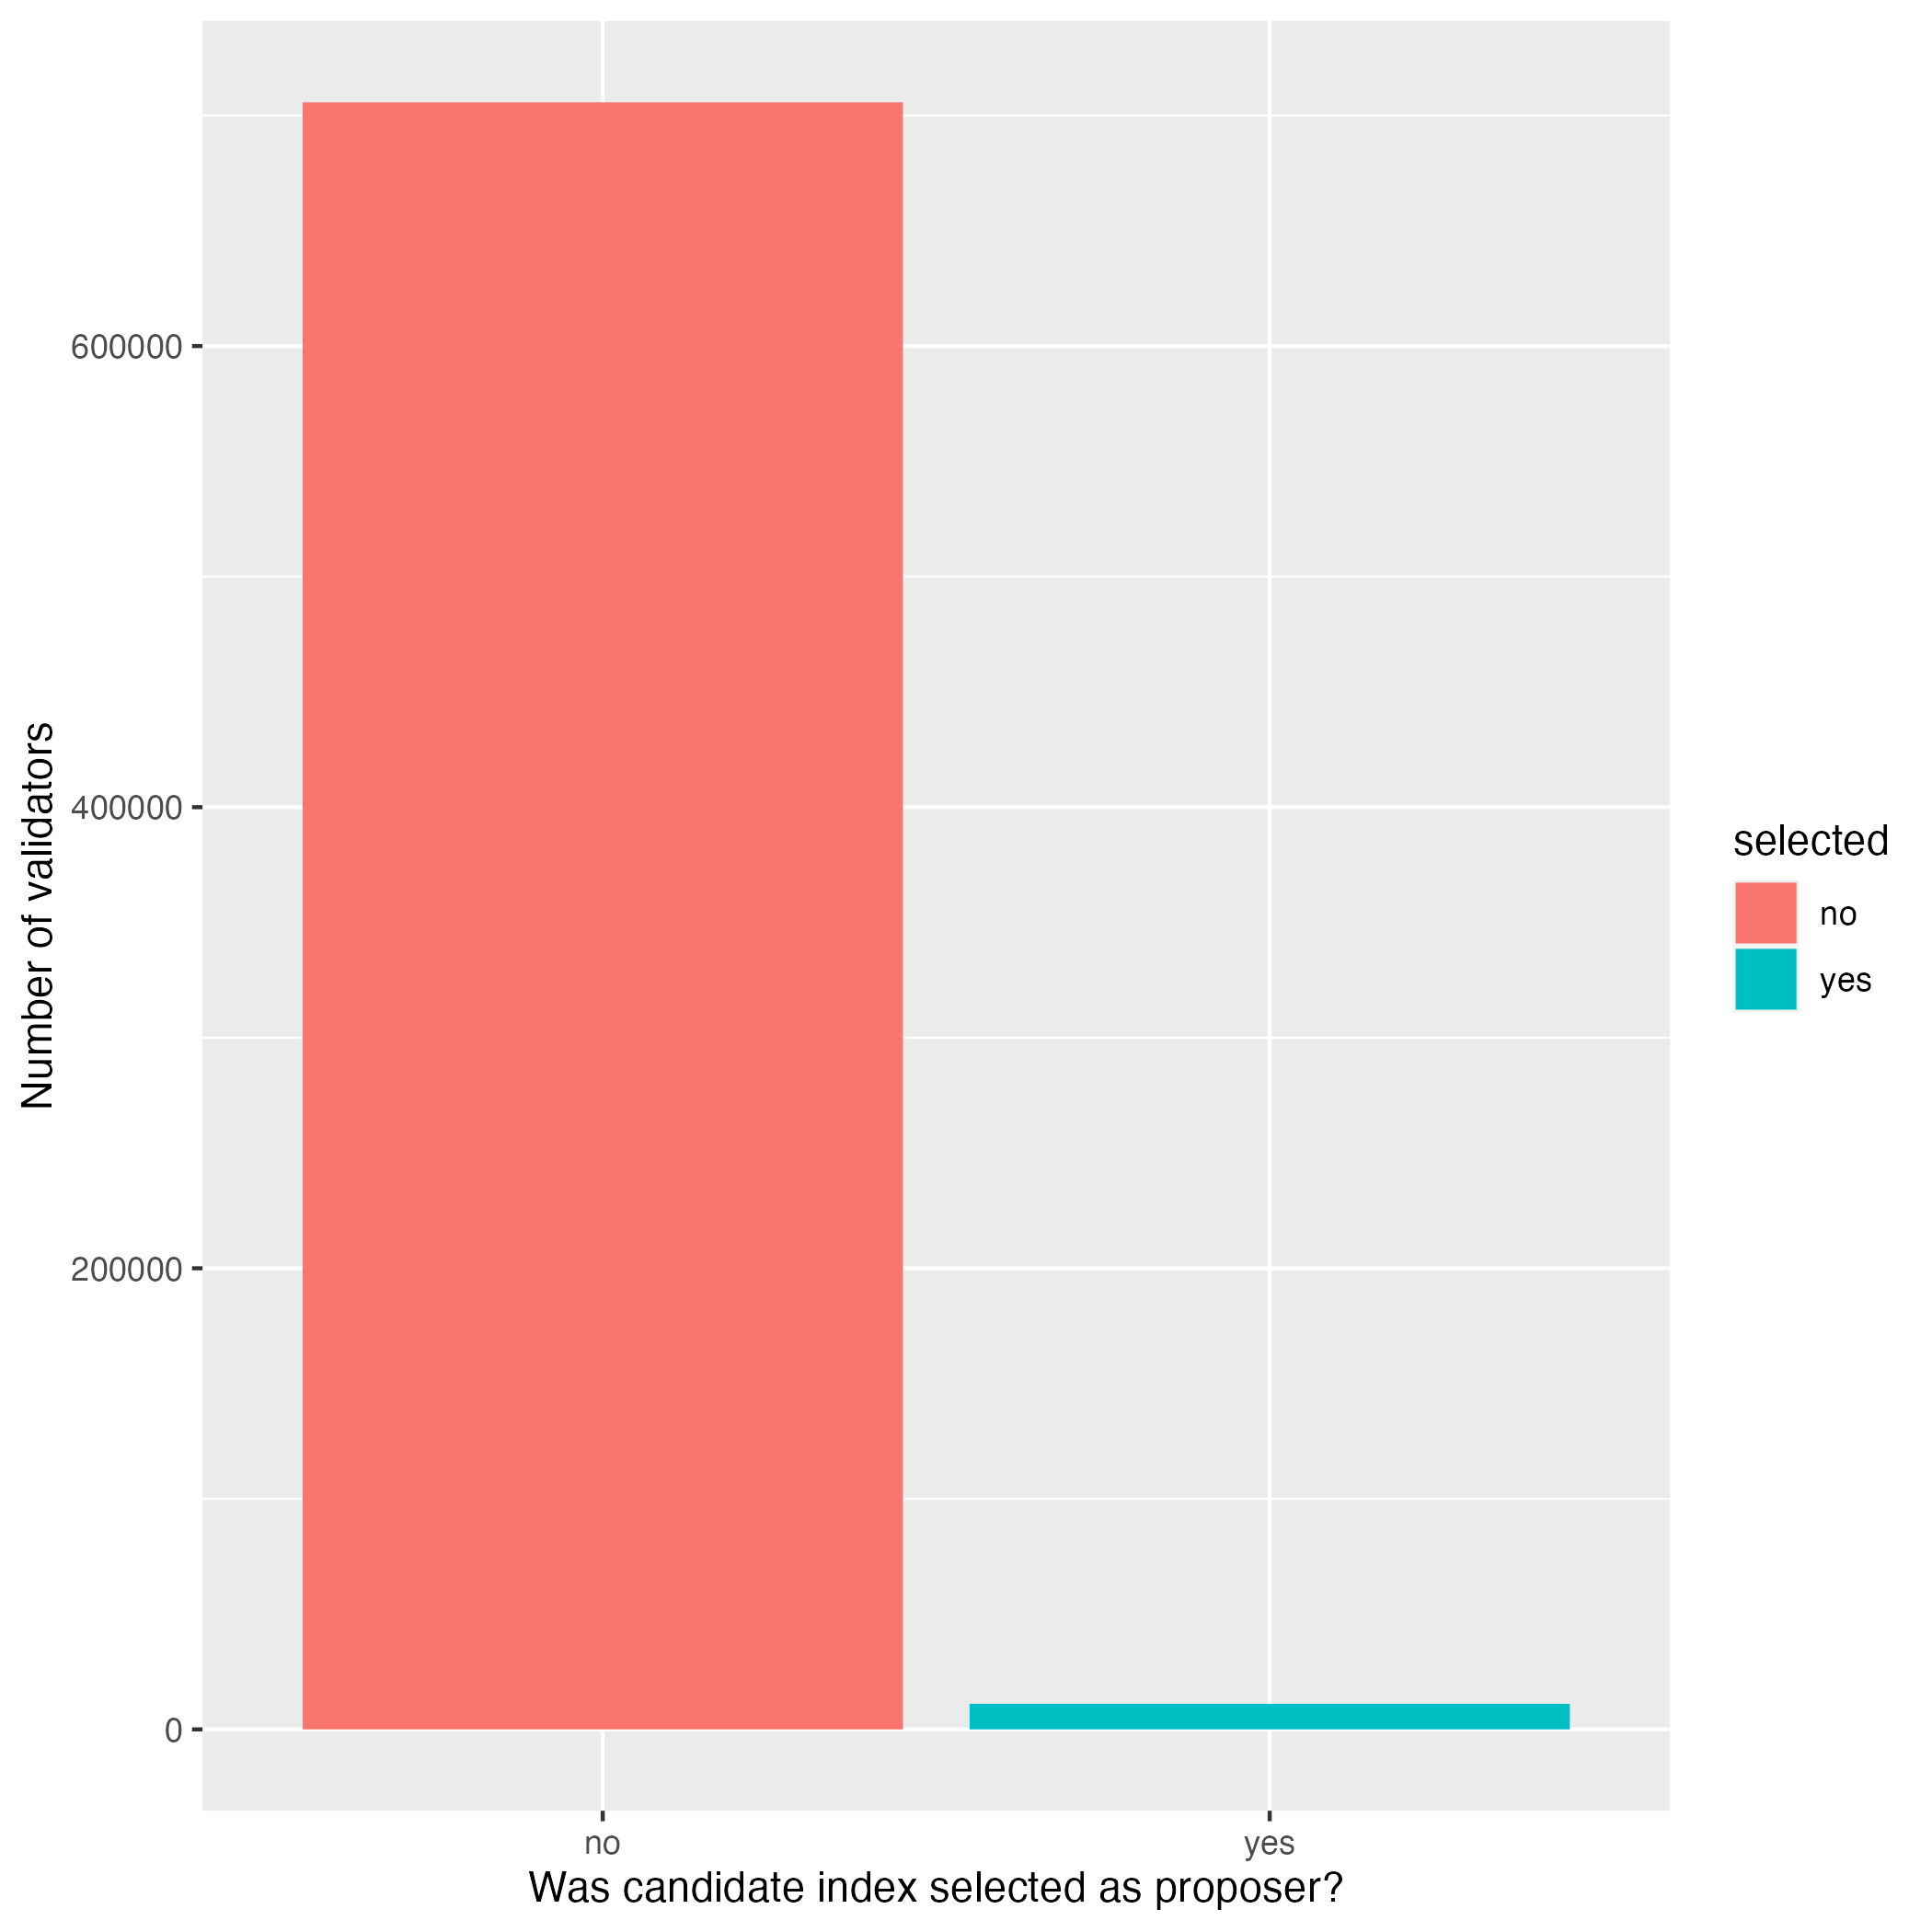
\includegraphics[width=0.45\linewidth]{images/maxeb-solo-barchart} \\
(a) \hspace{180pt}     (b)
\caption{Proportion of validators with random byte that passes proposer check if all validators have 32 ETH effective balance, and (a) maxEB = 32 ETH, (b) maxEB = 2,048 ETH}
\label{fig:maxebsolo}
\end{center}
\end{figure}

\noindent
\textbf{\textit{Scenario 2}} \\
% -------------------
\noindent
In this scenario we have full consolidation by all stakers, so probabilities and mechanisms for selection remain unchanged, i.e. when a candidate validator's balance = maxEB, then they will be selected with certainty, i.e. a probability of 1. \\

\clearpage
\noindent
\textbf{\textit{Scenario 3}} \\
% -------------------
\noindent
A more interesting scenario is when we look at a variety of effective balances. As an example, let us assume that the validator set of 716,800 validators is made up of a combination of consolidation options as shown in Table \ref{tbl:scenario3} on page \pageref{tbl:scenario3}. Based on this chosen configuration, the total validator set size reduces to 297,248: \\

\noindent
\textit{Number of single validators} $= \frac{716,800 * 0.30}{1} = 215,040 $ \\
\textit{Number of 64ETH validators} $= \frac{716,800 * 0.20}{2} = 71,680 $ \\
\textit{Number of 320ETH validators} $= \frac{716,800 * 0.10}{10} = 7,168 $ \\
\textit{Number of 2,048ETH validators} $= \frac{716,800 * 0.30}{64} = 3,360 $ \\
\textit{Adjusted validator set after consolidation}$ = 215,040 + 71,680 + 7,168 + 3,360 = 297,248$ \\

\noindent
 We calculate the probability that a validator is selected and passes the check for proposer eligibility, as the product of the probability of being the candidate index  and the probability of passing the proposer check, since these two events are independent, i.e. $P(A \cap B) = P(A/B)P(B) = P(A)P(B)$. Using the logic from equation \ref{eqn:1} and the example calculations that followed, we populated the table accordingly.
\begingroup
\renewcommand{\arraystretch}{1.5} % Default value: 1
\begin{table}[htp]
\caption{Active validator set composition for Scenario 3}
\label{tbl:scenario3}
\begin{center}
\begin{tabular}{|c|c|c|c|c|c|}
\hline
\textbf{Staker} & \textbf{\% of total} & \textbf{Effective} & \textbf{P(candidate)} & \textbf{P(proposer} & \textbf{P(candidate} \\
\textbf{Consolidation} & \textbf{deposit } & \textbf{balance} &\textbf{ } & \textbf{check = Y) } & \textbf{ \& selected)} \\
\hline
Single & 30\% & 32 ETH & $\frac{215,040}{297,248} = 0.723$ & 0.016 & $0.723*0.016 = 0.0116$\\
Partial (2-fold) & 20\% & 64 ETH & $\frac{71,680}{297,248} = 0.241$ & 0.031 & $0.241*0.031 = 0.0075$\\
Partial (10-fold) & 10\% & 320 ETH & $\frac{7,168}{297,248} = 0.024$ & 0.156 & $0.024*0.156 = 0.0037$\\
Fully (64-fold) & 30\% & 2,048 ETH & $\frac{3,360}{297,248} = 0.011$ & 1.000 & 0.0113*1.000 = 0.0113 \\
\hline
TOTAL & 100\% & \texttt{ } & 1.00 & \texttt{ } &  \texttt{ } \\
\hline

\end{tabular}
\end{center}
\end{table}%
\endgroup

The above scenario tells an interesting story. If the lion share of the total stake is shared equally between single and fully consolidated validators, then it is equally likely for either category to be selected as a proposer of the next block. The varying proportions of, and extent of, consolidation would appear to be less desirable, but we need to put these observations in the context of the total stake for each of the categories in the scenario. \\

Taking a very simple example, say we have a validator set size of 100, where 32 validators are run by single stakers, and there is 1 large staker running 64 validators. The large staker decides to consolidate all 64 validators into one `super' validator. Then the probability of the large staker's validator being selected as the candidate index for proposing the next block is $\frac{1}{33} = 0.03$, where previously it would have been $\frac{64}{100} = 0.64$ that one of its validators would be the candidate index selected. Once the check for proposer eligibility is made, the super validator will always pass that check, i.e. probability of 1. For a solo validator to be the selected candidate index would also be 0.03, but the probability that one of the solo stakers is selected, rather than a super validators is $\frac{32}{33} = 0.97$.

\noindent
\clearpage

\textbf{\textit{Proposer Bayesian network}} \\
% -------------------
\noindent
Building on Scenario 3, we can develop a simple Bayesian network (BN)  to explore the consequences of various choices. The total number of validators before any consolidation of stake is assumed to be 716,800.  Moreover, we will make some assumptions about a possible distribution of consolidated and single validators for various categories of staker. All these assumptions can be replaced with alternative assumptions in the BN. 

The following tables describe the key factors (nodes) in the BN and the probability table attached to each node. Figures xx to zz depict the BN structure and the resulting marginal probabilities when we run the network.
 
 \begin{table}[htp]
\caption{Staker categories}
\begin{center}
\begin{tabular}{|l|l|c|}
\hline
\textbf{Category} & \textbf{Description} & \textbf{Proportion of} \\
 & & \textbf{validator set} \\
 \hline
Small-scale solo stakers & 32 - a few hundred ETH & 0.30 \\
Large-scale individual solo stakers & 1000+ ETH & 0.15 \\
Large-scale institutional solo stakers & companies staking their own ETH & 0.15 \\
Centralized staking pools & & 0.10 \\
Semi-decentralized staking pools & Rocketpool, Lido... each one is different & 0.30 \\
\hline
\end{tabular}
\end{center}
\label{tbl:stakers}
\end{table}%


\begingroup
\renewcommand{\arraystretch}{1.5} % Default value: 1
\begin{table}[htp]
\caption{P(validator selected as candidate proposer)}
\label{tbl:candidate}
\begin{center}
\begin{tabular}{|c|c|c|c|}
\hline
\textbf{Validator} & \textbf{Marginal} & \textbf{Number of} & \textbf{P(selected as} \\
\textbf{consolidation} & \textbf{probability } & \textbf{validators} &\textbf{ candidate)}  \\
\hline
Single & 28.75\% & $\frac{0.2875 * 716,800}{1} = 206,080$ & $\frac{206,080}{329,810} = 0.6248$ \\
Partial (2-fold) & 25.75\% &  $\frac{0.2575 * 716,800}{2} = 92,288$ & $\frac{92,288}{329,810} = 0.2798$ \\
Partial (5-fold) & 15.00\% &  $\frac{0.1500 * 716,800}{5} =  21,504$ & $\frac{21,504}{329,810} =  0.0652$ \\
%Partial (10-fold) & 9.00\% &  $\frac{0.0900 * 716,800}{10} = 6,451.2$ & $\frac{6,451.2}{329,810} = 0.0196$ \\
Partial (10-fold) & 9.00\% &  $\frac{0.0900 * 716,800}{10} = 6,451$ & $\frac{6,451}{329,810} = 0.0196$ \\
%Partial (30-fold) & 8.50\% &  $\frac{0.0850 * 716,800}{30} = 2,030.93$ & $\frac{2,030.93}{329,810} = 0.0062$ \\
Partial (30-fold) & 8.50\% &  $\frac{0.0850 * 716,800}{30} = 2,031$ & $\frac{2,031}{329,810} = 0.0062$ \\
Fully (64-fold) & 13.00\% &  $\frac{0.1300 * 716,800}{2,048} = 1,456 $ & $\frac{1,456}{329,810} =  0.0044$\\
\hline
TOTAL & 100\% & 329,811 & 1.0000 \\
\hline

\end{tabular}
\end{center}
\end{table}%
\endgroup

Note that the probability that any one validator in the heterogeneous validator set is selected is $\frac{1}{329,810} = 0.000003$, but the probability that the validator belongs to a certain `type' of validator differs as shown in Table \ref{tbl:candidate}. Similarly, the probability that a validator from a particular staker is selected as the candidate index is proportional to the number of validators in the active validator set, regardless of whether it is consolidated or not.

\clearpage
% ------------------------------------------------
\subsubsection*{Sync committee}
% ------------------------------------------------
As discussed in the \href{https://ethresear.ch/t/increase-the-max-effective-balance-a-modest-proposal/15801/3}{blog post}, the expectation is that this selection process will work as designed even when there is a large increase in Max\gls{eb} \cite{Neuder2023a}.

Sync committee members are selected with replacement from the active validator set. The probability of being selected is proportional to the ratio of the validator's effective balance, i.e. the number of increments, \textit{n}, to the total number of increments in the validator set, \textit{T}, i.e. $\frac{n}{T}$ \cite{Edgington2023}. 

The denominator for the acceptance probability is MaxEB which means the probability will change from $\frac{b}{32}$ to $\frac{b}{2,048}$, where \textit{b = validator effective balance}. Check whether this adversely affects validators with a small stake, apart from the expected increase in time to select the committee, as D'Amato and Neuder pointed out \cite{damato2023}.
% ------------------------------------------------
\subsubsection*{Slot committees}
% ------------------------------------------------
Selection of the 32 slot committees for each epoch does not take validator effective balance into account. However, when single slot finality is implemented, the fact that different committees may have different weights would not be relevant since all the active stake will vote in each slot.

Currently, however, the weight distribution across slot committees could vary, depending on the percentage of membership of the committees with partially or fully consolidated validators.
% ------------------------------------------------
\subsubsection*{Aggregators}
% ------------------------------------------------
For the \href{https://eth2book.info/capella/part2/building_blocks/aggregator/}{existing distribution of the expected number of aggregators} per sub-committee, refer to Edgington's online book \cite{Edgington2023}.
If more than one of the virtual validators of a consolidated validator is chosen, then it is still just that one validator in the set of aggregators. 

% ------------------------------------------------

% ------------------------------------------------
% -----------------------------------------------------------
\subsection{Analysis of Rewards \& Penalties}
% -----------------------------------------------------------
\subsubsection{Rewards}
% ------------------------------------------------
Elowsson (2024) published a comprehensive post on ethresear.ch on Ethereum issuance. This post included analysis and modelling of consensus incentives and variability of solo staker reward, as well as several other aspects relevant to issuance and staker yield (\href{https://ethresear.ch/t/properties-of-issuance-level-consensus-incentives-and-variability-across-potential-reward-curves/18448}{Properties of issuance level: consensus incentives and variability across potential reward curves}).

\noindent
\textbf{Proposer rewards} \\
% ------------------------------------------------

\noindent
\textit{Proposer award for attestations} \\
% ------------------------------------------------


\noindent
\textit{Proposer award for sync committees} \\
% ------------------------------------------------




\noindent
\textbf{Attestation rewards} \\
% ------------------------------------------------



\noindent
\textbf{Whistleblower reward} \\
% ------------------------------------------------


\noindent
\textbf{Sync committee rewards} \\
% ------------------------------------------------


% ------------------------------------------------
\subsubsection{Penalties}
% ------------------------------------------------
% ------------------------------------------------
\textbf{Slashing penalties} \\
% ------------------------------------------------
\noindent
Listed below are links to posts about slashing penalties, the effect on them when EIP-7521 is implemented, including some proposals for modifications to existing penalties:
\begin{enumerate}
\item \href{https://a16zcrypto.com/posts/article/the-cryptoeconomics-of-slashing/}{The cryptoeconomics of slashing} by Kannan and Deb.
\item \href{https://ethresear.ch/t/slashing-penalty-analysis-eip-7251/16509}{Slashing penalty analysis} by Neuder and Monnot.
\item \href{https://notes.ethereum.org/@mikeneuder/slashings-eip-7251}{DRAFT] Slashing penalty analysis; EIP-7251} by Neuder and Monnot.
\item \href{https://hackmd.io/@dapplion/maxeb_slashing_risks}{MaxEB slashing risks} by dapplion
\item \href{https://colab.research.google.com/drive/1lBe4qH4oqI8D9cmcQGca3O1AdR3SVr5z?usp=sharing#scrollTo=Hiw1NPEZIQVi}{Slashing simulation code}
\end{enumerate}


\noindent
In the $3^{rd}$ blogpost, Neuder and Monnot propose the following for current slashing penalties \cite{Neuder2023d}: 
\begin{itemize}
\item Changes to existing penalties:
	\begin{itemize}
	\item Changing the \textit{initial penalty} to be either fixed, or scaled sublinearly
	\item Changing the \textit{correlation penalty} to scale quadratically rather than linearly.
	\end{itemize}
\item Unchanged penalties:
	\begin{itemize}
	\item \textit{Attestation penalties}
	\item \textit{Inactivity leak penalties}
	\end{itemize}
\end{itemize}

\noindent
\textbf{\textit{Initial slashing penalty}} \\
% -------------------------------------------------
The initial slashing penalty is proportional to the validator's effective balance, $MIN\_SLASHING\_PENALTY\_QUOTIENT\_BELLATRIX=32$, giving a maximum penalty of 1 ETH if the slashed validator has 32 ETH, the current MaxEB.
If left unchanged, a fully consolidated validator would incur an initial slashing penalty of 64 ETH. There appears to be general agreement that this initial penalty is too high, and may deter larger stakers such as Lido to support EIP-7521.

Neuder and Monnot suggest that the initial penalty could either be changed to a constant value, or through a monotonically increasing function, e.g.  from the family of polynomials. The latter appears to be the preferred option. However, mention has also been made of a zero initial slashing penalty since a slashed validator already incurs additional penalties such as attestation penalties and lost revenue while waiting for its exit epoch. Francesco is not in favour of a zero initial penalty because that means that there is no penalty to proposal equivocation, which is already a relatively cheap \gls{dos} attack vector on the network. For example, it is not good if someone can make 1,000 different blocks at zero cost.

For a monotonically increasing function, the authors propose the following function to calculate the revised initial slashing penalty:\\
\textit{initial penalty =} $\frac{EB^x}{32}, \texttt{ } x \leqslant 1$ \\

Their blogpost has graphs for $x=1, \frac{15}{16}, \frac{7}{8}, \frac{3}{4}, \frac{1}{2}$ and a line for a constant initial penalty of 1 ETH \cite{Neuder2023d}.

The authors conclude that visually it appears that $x = \frac{3}{4}$ and $\frac{7}{8}$ are good choices in terms of balancing the size of the initial slashing penalty and the risk for a consolidated validator.\\

Since the previous discussion and reasoning, an alternative point of view has been put forward, and that is to set the initial slashing penalty to zero. LIDO appears in favour of a small penalty as a deterrent, but penalties are already incurred due to the enforced wait time to the exit epoch and a small or zero initial penalty would not seem all that relevant. Moreover, a zero initial slashing penalty would favour smaller stakers over larger stakers.

Lion commented that setting the initial slashing penalty to zero does not fix the original aim of splitting attester and proposer slashing.  Although not specifically related to MaxEB, Lion summarised discussion around proposer and attester slashing in the following \href{https://docs.google.com/document/d/1mOc5nokVm3jx4bCffTuQ_xjYV4zVlDLPI-KEhFWWP78/edit}{blog post}.

\noindent
\textbf{\textit{Correlation penalty}} \\
% --------------------------------------------
This penalty is incurred roughly 18 days (4,096 epochs) after the slashing event, half way between its exit epoch and the slashing event \cite{Edgington2023}. The correlation penalty is important in penalising apparent coordinated attacks on the chain, and is the only other penalty that Neuder and Monnot propose to alter \cite{Neuder2023d}.

The penalty for a slashed validator is calculated as follows using the previous 36 days from this ``half-way'' epoch.
\begin{equation*}
\begin{split}
& \textit{correlation penalty} = \left\lfloor \frac{3*EB*SB}{TB} \right\rfloor, \texttt{ } where \\
& 3 = \textit{Bellatrix multiplier} \\
& EB = \textit{slashed validator's effective balance} \\
& SB = \textit{total slashable balance} \\
& TB = \textit{total effective balance of the beacon chain} \\
& \therefore \textit{if SB} = \frac{1}{3} * TB \implies \textit{ correlation penalty} = EB \\
& \textit{Similarly, if } 3*EB*SB <  TB \implies penalty = 0 \textit{ due to integer division} \\
\end{split}
\end{equation*}

There is currently no correlation penalty for isolated slashing events and this continues to be the case for a fully consolidated validator with 2,048 ETH effective balance as shown below using 24 million ETH as the total staked ETH, (\textit{TB}):

\begin{equation*}
\begin{split}
& \textit{ SB = EB for an isolated slashing} \\
& \therefore  3*EB*SB =  3*EB*EB \\
& \textit{Assuming EB = 2,048 \& TB } = 2.4 * 10^7, \textit{ then} \\
& 3*EB*EB = 1.2582912 * 10^7 < 2.4 * 10^7 \\
& \therefore penalty = 0
\end{split}
\end{equation*}

For EIP-7521 the authors propose a function that preserves the requirement that when the total slashed balance is $\frac{1}{3}^{rd}$ of the total balance, the entire balance of the validator is slashed:

\begin{equation*}
\begin{split}
& penalty' = \frac{3^2 * EB * SB^2}{TB^2} \\
& \therefore \textit{if SB } = \frac{TB}{3}, \textit{ then} \\
& penalty' =   \frac{3^2 * EB * \left(  \frac{TB}{3} \right)^2 }{TB^2} \\
& \therefore penalty' = EB
\end{split}
\end{equation*}

Moreover, the new correlation penalty function scales quadratically as opposed to the current function that scales linearly. With the proposed new function, the slashing penalties are substantially reduced for all validators, regardless of whether they have consolidated stake.

Refer to the \href{https://notes.ethereum.org/@mikeneuder/slashings-eip-7251}{blogpost} to view graphs showing the comparative correlated slashing penalties for solo (32 ETH), partially consolidated (256 ETH), and fully consolidated (2,048 ETH) validators applying both the current and the proposed functions \cite{Neuder2023d}. \\

Lion summarised some discussion around proposer and attester slashing, with the aim of decoupling correlated penalties from equivocating proposers and reducing a validator's time in exit status. (\href{https://hackmd.io/@dapplion/S1pGYKR_T}{blog post}). Independence is required for message replay protection. By reverting this \gls{pr} consolidated validators have a higher expected cost of proposer errors. However, the expected cost is negligible. If large stakers are convinced of this, then the additional complexity can be removed and Lion is in favour of dropping it.

In other words, by setting the initial penalty to 0 and keeping the separation of proposer and attester slashing, the cost of proposer equivocation becomes very low. Agreement whether the additional complexity in the slashing flow is justified is still uncertain. It seems that the main benefit is when there are high correlation penalties (which will also affect staking pool validators), or very long exit queues, e.g. several months. At other times the cost is merely missed revenue plus penalties accrued over the 36 day withdrawal period, i.e. $\frac{1}{6}^{th}$ if the yield, like $0.5\%$ now.



\noindent
\textbf{\textit{Attestation penalty}} \\
% -----------------------------------------
Once a validator is slashed, their attestations (source, target and head votes) are deemed to be invalid and hence they incur attestation penalties for 8,192 epochs until their exit epoch. 

Different weights are attached to each vote, but only the source (weight = 14) and target (weight = 26) votes incur penalties. For each of the 8,192 epochs the slashed validator will incur:

\begin{equation*}
\begin{split}
& Given:\\
& \textit{base reward} = \frac{64}{ \left\lfloor \sqrt{TB} \right\rfloor} \textit{, weight denominator} = 64, \\
& \textit{source weight} = 14 \textit{  \& target weight} = 26\\
& \\
& \therefore \textit{epoch attestation penalty} = \frac{\textit{base reward} * EB * (14 + 26)}{64} \\
& \therefore \textit{ if } TB \approx 24 \textit{million ETH} = 2.4 * 10^6 * 10^9 \textit{ Gwei}\\
& \textit{the integer square root of } 2.4 * 10^6 * 10^9 \textit{ Gwei} = 154,919,333 \\
& \textit{base reward} = \frac{64 * 10^9}{154,919,333} = 413 \textit{ Gwei} \\
& \\
& \therefore \textit{for a \textbf{solo staker} with 32 ETH:} \\
& \textit{total attestation penalty for 8,092 epochs} = 8192 * \frac{413*32*40}{64}  \textit{ Gwei}  \approx 0.06767 \texttt{ } ETH \\
& \textit{for a \textbf{fully consolidated} validator with 2,048 ETH:} \\
& \textit{total attestation penalty for 8,092 epochs} = 8192 * \frac{413*2048*40}{64}  \textit{ Gwei}\approx 4.331 \texttt{ } ETH \\
\end{split}
\end{equation*}

This attestation penalty for a large slashed staker seems acceptable, but could potentially be adjusted by changing the number of epochs that the validator is deemed as being ``offline''.The size of this penalty needs to be such that the security model is not compromised. In other words it should never be a better option to self-slash to avoid inactivity penalties. Therefore, it needs to be greater than the inactivity penalties for an unslashed validator that is exiting and offline \cite{Neuder2023d}. \\

\noindent
\textbf{\textit{Inactivity leak penalty}} \\
% -------------------------------------------------------------------
An \textit{inactivity leak} is signalled by the protocol when the chain has not been finalising for 4 epochs. During an inactivity leak online validators will not penalised, so although no rewards are being earned, the penalty is 0. 

On the other hand, offline validators, which includes slashed validators waiting to exit, start `leaking' state. The loss of stake means that the relative weight of the online validators will increase, which helps the chain to start finalising again. The inactivity penalty can be quite severe. 

Using the current method, the authors calculated the penalty for three different effective balances: 32 ETH (solo validator), 256 ETH (partially consolidated validator),  and 2,048 ETH (fully consolidated validator).

\begin{table}[htp]
\caption{Inactivity leak penalties}
\begin{center}
\renewcommand{\arraystretch}{1.3}
\begin{tabular}{|l|l|l|l|}
\hline
\textbf{validator size} & \textbf{16 epoch leak} & \textbf{128 epoch leak} & \textbf{1024 epoch leak} \\
\hline
32 ETH & 0.000259 ETH & 0.0157 ETH & 1.00 ETH \\
256 ETH & 0.00208 ETH & 0.126 ETH & 8.01 ETH \\
2048 ETH & 0.0166 ETH & 1.01 ETH & 64.1 ETH \\
\hline
\end{tabular}
\end{center}
\label{default}
\end{table}%

\noindent
\textbf{\textit{Potential slashing during consolidation}} \\
\label{consolidationslashing}
% -------------------------------------------------------------------
The points summarised here arose from discussions amongst several people, including Lion, Mikhail Kalinin, Francesco, Barnabé Monnot, Mike Neuder, Roberto Saltini.

Importantly, we need to assess what effect the implementation of EIP-7521 could have on the risk of being slashed.

As mentioned earlier Lion created a model for slashing risk profile. The link to the \href{https://colab.research.google.com/drive/1lBe4qH4oqI8D9cmcQGca3O1AdR3SVr5z?usp=sharing}{source Python code} has edit permissions, with an accompanying document on \href{https://hackmd.io/@dapplion/maxeb_slashing_risks}{MaxEB Slashing Risk}. \\

\noindent
\textbf{Scenarios}: 
\begin{enumerate}
\item Validation keys are stolen\\
\\
The balance is secured by withdrawal credentials, therefore malicious consolidation is not anticipated to be valuable for an attacker. \\
\\
Nonetheless, it would be helpful to know how pools manage withdrawals. To the best of our knowledge LIDO has single withdrawal credentials for all validators, and Rocket Pool different withdrawal credentials for each validator. On the other hand, centralised stakers, such as Coinbase, apparently try to obfuscate and will therefore probably have different sets of credentials.

\item Chain forks during consolidation of validators \\
\\
It is vital that we keep track of slashing across both the source and target for consolidation, rather just one or the other. Francesco demonstrated the need for this by visualising the scenario in figure~\ref{fig:francesco1} on page \pageref{fig:francesco1}. The scenario is described below.
\end{enumerate}

\begin{figure}[htbp]
\begin{center}
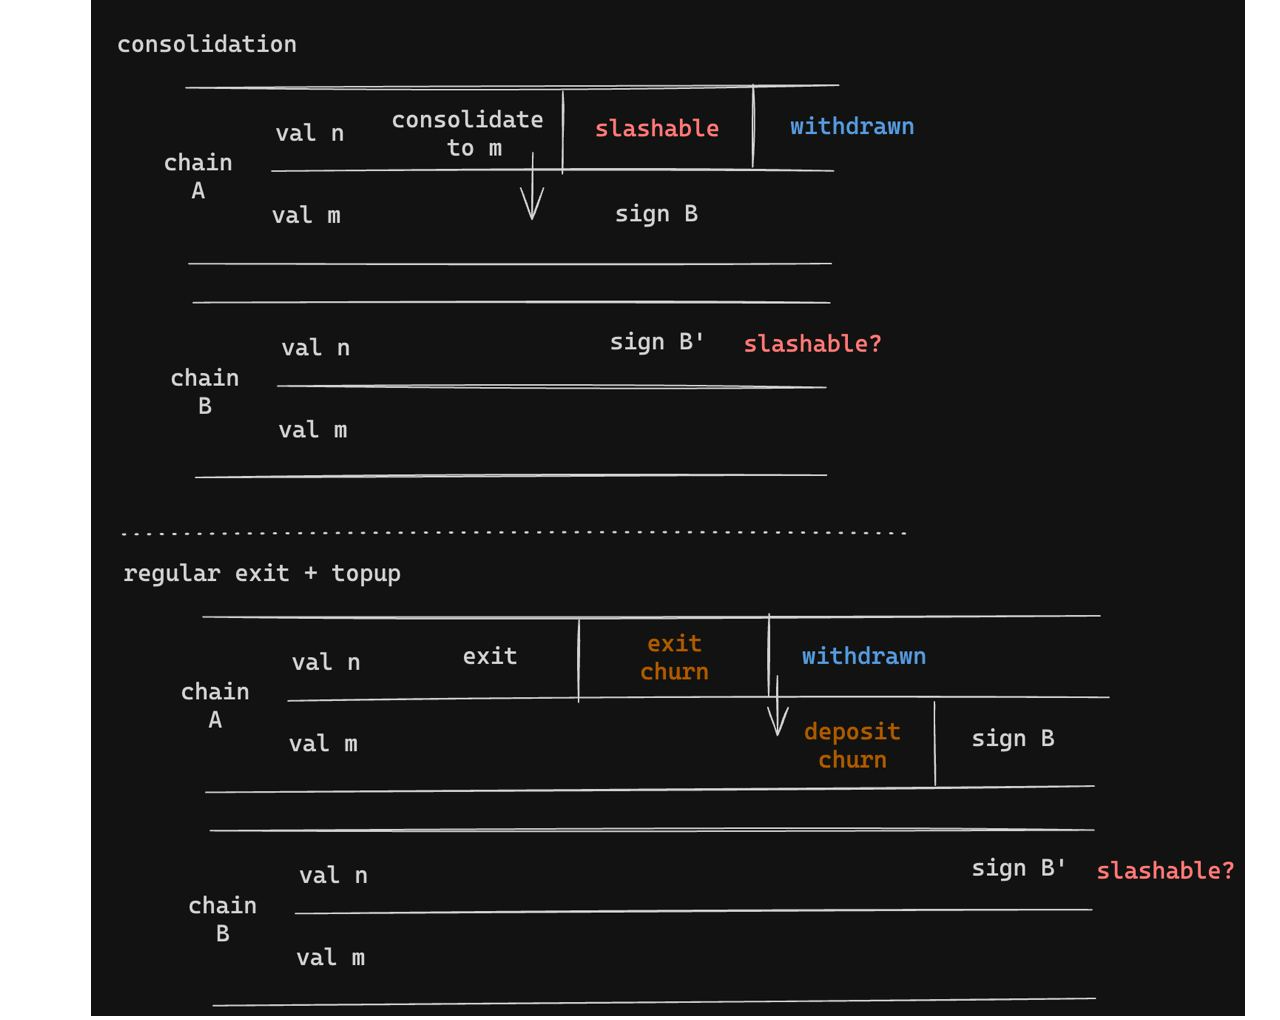
\includegraphics[width=0.7\linewidth]{images/francesco1}
\caption{A fork where consolidation is yet to occur and one where it has happened}
\label{fig:francesco1}
\end{center}
\end{figure}

\noindent
\textbf{Scenario 2 - fork during consolidation} \\
In figure~\ref{fig:francesco1} we see that validator \textit{n} consolidates to validator \textit{m} on chain \textit{A}, but not on chain \textit{B}. 

Validator \textit{n} then signs two different blocks at the same slot, or does surround voting, in a way that is not deemed to be slashable in the existing consolidation \gls{pr}. Based on this potential scenario, Francesco wondered if it would be that complicated to enable slashing ``across consolidations''.

Mikhail replied that this would be possible, providing that chain \textit{B} is aware that the consolidation happened on chain \textit{A}. Moreover, a slasher would need to resolve the final consolidation index in order to detect a new source of slashable offences between the source and target of consolidated validators.

Mikhail suggested three options to enable slashing across consolidations:
\begin{enumerate}
\item pass the consolidating stake through the activation churn.\\
\\
Bypassing the exit churn would be the improvement for stakers and a consolidation to be reverted if the source is slashed before the \gls{eb} was fully activated, without the necessity to make the target liable for the source's slashings.\\
Mikhail feels that this option is more natural from the protocol perspective. Consolidating via churn when the queue is empty means it will be 4 epochs, instead of 2 epochs to wait for consolidation to be finalised. However, Francesco pointed out that a large amount of consolidations would require weeks or months of churn.  Nonetheless, Mikhail does not expect pools to consolidate much faster than allowed by the churn due to the inherent risks. The concern is that pools would be reluctant to consolidate via churn due to lost revenue. 

\item finalise consolidation on-chain before activating a consolidated balance. This is akin to waiting for \textit{activation\_eligibility\_epoch} to be finalised. \\
\\
This is Mikhail's preferred option, with the addition of improving the slasher's design.
\item accompanying the slashing message with the consolidation from another chain.
\end{enumerate}

Mikhail summarised the proposed slashing rule for a consolidation event is as follows: \\
\noindent
Resolve the final target validator and slash the whole consolidation chain: the source, interim targets and the final target.

From the perspective of the slasher, the slashable offence occurs whenever \textit{consolidated\_to} is changed on any of the observable forks. 



% ------------------------------------------------

% ------------------------------------------------
\subsection{Analysis of Ethereum ecosystem \& protocol}
% -------------------------------------------------------------------------
% ------------------------------------------------------------
\subsubsection{Worst case: Full consolidation}
% -------------------------------------------------------------

% ------------------------------------------------------------
\subsubsection{Griefing / Discouragement attacks}
% -------------------------------------------------------------
According to Buterin a griefing attack is when a validator acts maliciously inside a consensus mechanism to reduce other validators' revenue even at some cost to themselves to encourage the victims to drop out of the mechanism \cite{buterin2018c}.

The two main motivations for reducing the number of participants are most likely because fewer participants:
\begin{itemize}
\item mean greater rewards for those remaining in the mechanism
\item helps to prepare an attack on the chain by reducing the cost of an attack
\end{itemize}

Some strategies have already been put in place to avoid discouragement attacks \cite{Edgington2023}:
\begin{itemize}
\item inverse square root scaling of validator rewards
\item scaling of rewards with participation (viz. for each ``source, target, and head vote, the attester's reward is scaled by the proportion of the total stake that made the same vote'')
\item zeroing attestation rewards during an inactivity leak
\item rate limiting of validator exists, which means that an attacker needs to sustain an attack for longer and at greater cost in order to achieve the same outcome.
\end{itemize}

% ------------------------------------------------------------
\subsubsection{Consolidation of validators}
% -------------------------------------------------------------
Slashing as a direct result of consolidation of validators is discussed in \ref{consolidationslashing}. The example given is when the consolidation event occurs during a fork in the chain.

Mike Neuder had a proposal that did not get much traction, but that sounded interesting:\\
\begin{itemize}
\item Have a one-time consolidation event
\item A hot update of validator balances during the hard fork on pre-signed messages 
\end{itemize}
If this was an option then there would be no ip merge needed and we have people committing to merging validators.

Lion thought it was an interesting idea, but not sure if such an event would negate consolidation concerns. It appears that Francesco was also not in favour of such a proposal, but unsure of the reasons why.

% ------------------------------------------------------------
\subsubsection{Withdrawals}
% -------------------------------------------------------------
There is also discussion around how withdrawals for consolidated validators should work. There are two main ways of achieving this, and some stakers may want both, instead of settling for one of the two options:
\begin{itemize}
\item Custom ceilings
\item Partial withdrawals
\end{itemize}

The idea of custom ceilings is that a staker nominates a ceiling for a consolidated validator, and when that ceiling it reached, then the partial withdrawal sweep will move any balance above the ceiling into the validator's account. In other words it functions like the current withdrawal sweep, but in stead of kicking in at 32ETH balance for each validator, it will vary as specified for each consolidated validator.

The contention here is that custom ceilings add complexity to the protocol. which is unnecessary if partial withdrawals cover all the use cases.  However, \gls{el} partials are gas consuming, and from conversations that Mike Neuder had with staking pools, they prefer custom ceilings to partials. The added bonus is that it makes the change entirely a \gls{cl}  layer change.

Moreover the consolidation exercise is viewed as a one-off event meaning that there is no expectation that adjustments of ceilings should be catered for.

\subsubsection{Centralisation forces}
% ---------------------------------------------------------------
Historic and current trends for stake concentration are important to observe as these are warning signs that the chain is becoming more vulnerable to collusion. The consolidation of stake through EIP-7251 (currently in draft form) \cite{Neuder2023c} is unlikely to change the dynamics of stake concentration, since it is encouraging consolidation of validators already being operated by stakers. However, with more node operators and validators joining larger staking pools staked ETH will become more one-sided in favour of staking pools. 

% ------------------------------------------------

% ------------------------------------------------
% ------------------------------------------------
\subsubsection{Bayesian network model}
% ------------------------------------------------
We build a \gls{bn} model to capture the key factors and interactions for an increase in MaxEB as proposed in EIP-7521.

We assume that different groups, or categories, of stakers have different characteristics which will in turn influence their willingness to consolidate stake, as well as the uptake of validator consolidation. \\

\noindent
% ---------------------------------------------------------------
\textbf{Key factors} \\
% ---------------------------------------------------------------

\noindent
% ---------------------------------------------------------------
\textbf{Staker categories} \\
 % ---------------------------------------------------------------
Vitalik Buterin suggested potential categories as follows:
\begin{itemize}
\item Small-scale solo stakers (32 - a few hundred ETH)
\item Large-scale individual solo stakers (1000+ ETH)
\item Large-scale institutional solo stakers (ie. companies staking their own ETH)
\item Centralised staking pools
\item Semi-decentralised staking pools (Rocketpool, Lido... each one is different)
\item Each of the above, but using \gls{dvt}
\end{itemize}

Although each of the categories will differ with the use of \gls{dvt}, we do not anticipate that \gls{dvt} will influence their behaviour with respect to validator consolidation in any meaningful way. 

It will be challenging to assign a distribution across the proposed staker categories. However with current work on identifying validators, we would be able to assign some validators to staker categories and for those that are unknown, we can either replicate the distribution across the validators, or adjust them based on an assumption on the probability distribution across the unknown group. With the \gls{bn} we can also apply other distributions and see to what extent they affect the downstream probabilities. \\


\noindent
% ---------------------------------------------------------------
\textbf{Validator consolidation} \\
 % ---------------------------------------------------------------
 The implementation of EIP-7521 is likely to eventuate in a varying degree of consolidation within and across the various categories. We can use intuition for an initial uptake and vary this to test the downstream consequences of various scenarios.  \\
 
 \noindent
 % ---------------------------------------------------------------
\textbf{Health of the Ethereum ecosystem}
% ---------------------------------------------------------------
Ether alpha combines various aspects of the ecosystem to give an overall impression of the health of the network. They pull information from various sources for `Project Sunshine' dashboard \cite{easunshine}. 

The Rated network also provides detailed metrics and visualisations to gauge the health of the network \cite{Rated2023a}. 

 
 
 


% ------------------------------------------------


%\clearpage

\section{Bibliography}
% -----------------------------
\nocite{*}
\bibliographystyle{eptcs}
\bibliography{references}

\end{document}
